%!TEX root = ./../main.tex
\section{Einleitung}
Aufgabenstellung hier wiedergeben

\begin{itemize}
    \item Was ist Wikipedia?
    \item Wie viele Artikel, Edits, Autoren hat Wikipedia?\footnote{https://en.wikipedia.org/wiki/Wikipedia:Statistics}
    \item Ein Edit bzw. Update in Wikipedia wird durch ein neues Ereignis der realen Welt ausgelöst. Das kann eine Wahl,
    ein Unfall, politische Konflikte oder eine Sportveranstaltung sein \cite{10.1007978-3-642-36973-5_22}.
    \item Aufgabenstellung
    \begin{itemize}
        \item Für eine Entität (z. B. eine Person des öffentlichen Lebens) aus der Gesamtheite der Wikipedia-Edit-Events in "Echtzeit"
        Events der realen Welt ableiten.
        \item Wir betrachten nur die Metadaten (Zeitstempel, Autor, ...) und nicht den Inhalt der Änderung Änderung (z. B. textuelle Änderung).
        \item ...
    \end{itemize}
    \item Wie sieht so ein Burst of Wikipedia-Edits aus \ref{fig:donald_rumsfelds_resignation_burst}?
\end{itemize}


\begin{figure}[h]
    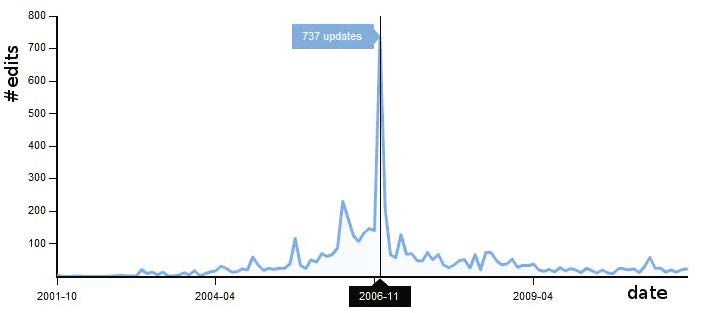
\includegraphics[width=.5\textwidth]{images/Extracting_EventRelated_Information_from_Article.jpg}
    \caption{Donald Rumsfeld’s Rücktritt führte zu einem Burst an Autoren, die einen Wikipedia-Edit vornahmen \cite{10.1007978-3-642-36973-5_22}.}
    \label{fig:donald_rumsfelds_resignation_burst}
\end{figure}